\chapter*{Введение}                         % Заголовок
\addcontentsline{toc}{chapter}{Введение}    % Добавляем его в оглавление

\newcommand{\actuality}{}
\newcommand{\progress}{}
\newcommand{\aim}{{\textbf\aimTXT}}
\newcommand{\tasks}{\textbf{\tasksTXT}}
\newcommand{\novelty}{\textbf{\noveltyTXT}}
\newcommand{\influence}{\textbf{\influenceTXT}}
\newcommand{\methods}{\textbf{\methodsTXT}}
\newcommand{\defpositions}{\textbf{\defpositionsTXT}}
\newcommand{\reliability}{\textbf{\reliabilityTXT}}
\newcommand{\probation}{\textbf{\probationTXT}}
\newcommand{\contribution}{\textbf{\contributionTXT}}
\newcommand{\publications}{\textbf{\publicationsTXT}}

Возникновение теории биологической эволюции берет свое начало в 18 - ом веке. Одним из первых, кто попытался выяснить как протекает процесс эволюции был выдающийся французский ученый - естествоиспытатель, Жан Батист Ламарк. Именно он в 1802 году впервые ввел термин ``биология''\,. В своем труде, ``Философия зоологии''\, \cite{Lamark} (1809), Ламарк утверждал, что движущими силами эволюции являются изменения окружающей среды.

В дальнейшем эта теория была развита Чарльзом Дарвином, английским натуралистом и путешественником, человеком, который вошел в историю как основоположник современной теории эволюции. Дарвином было проделано множество различных экспериментов, результатом которых стал его знаменитый труд --- ``Происхождение видов путем естественного отбора''\, \cite{Darwin} (1859). В этой работе были изложены три основных дарвинских принципа эволюции: наследственность, изменчивость и естественный отбор.  

\begin{figure}[ht]
\centerfloat{
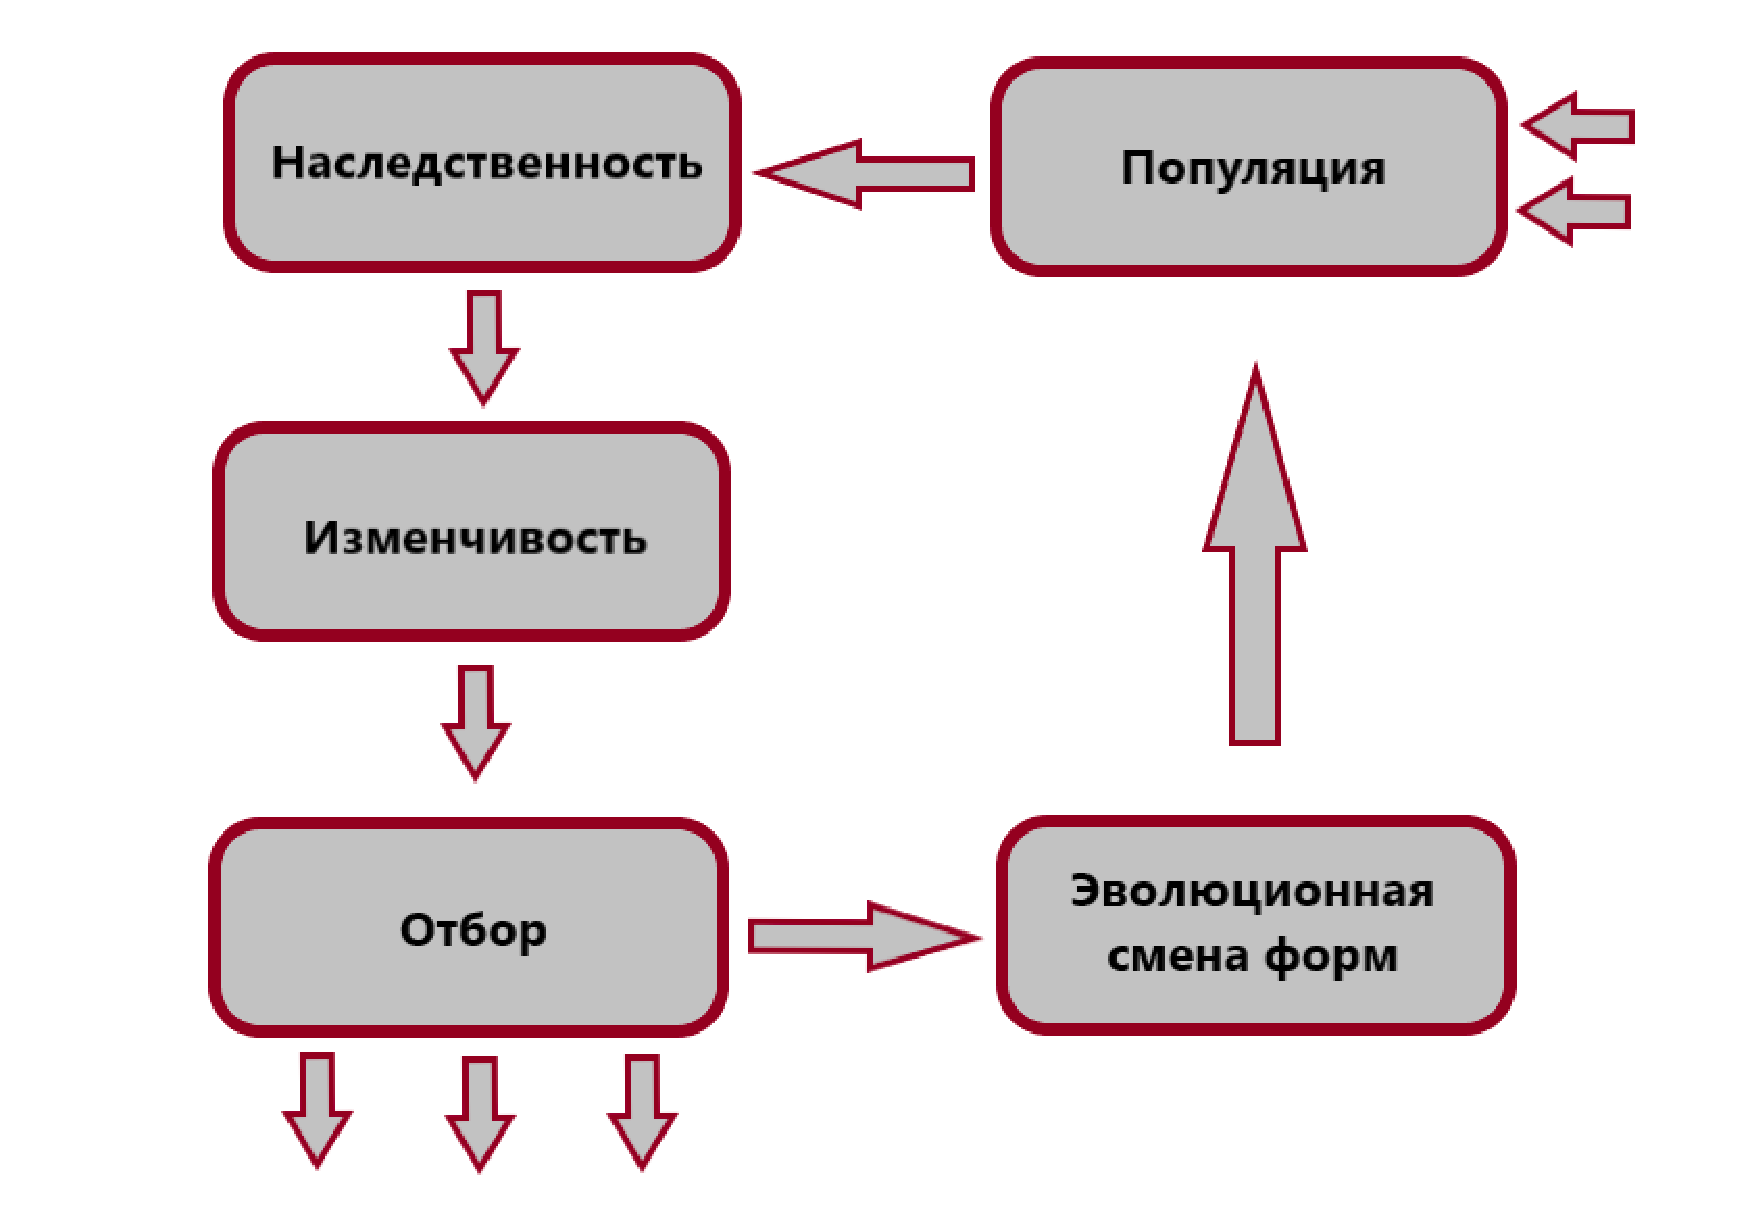
\includegraphics[width = 0.9\linewidth]{darwin.eps}
}
\caption{Схема эволюции Ч. Дарвина}
\label{fig1}
\end{figure}

Согласно Дарвину, живые организмы в течение всей своей жизни претерпевают различные мутации, которые могут быть обусловлены изменениями окружающей среды или возникновением конкуренции между соседствующими организмами. Это приводит к исчезновению старых признаков и появлению новых, более выгодных, которые затем наследуют потомки. Схематически принципы Дарвина можно изобразить так, как это показано на рис. \ref{fig1}.

Из личных записей Дарвина известно, что он читал работу Томаса Мальтуса --- автора теории ``народонаселения''\, или, как ее еще называют, теории ``Мальтузианства''\, \cite{Malthus}, опубликованную в 1978 году и был впечатлен полученными результатами. Основная идея теории Мальтуса заключалась в том, что в условиях неограниченности ресурсов, численность населения растет по закону геометрической прогрессии, в то время как скорость производства пищевых продуктов --- линейна. Результатом такого процесса является состояние, которое принято называть ``Мальтузианской ловушкой''\, (рис. \ref{fig2}), то есть ситуацией при которой численность населения превосходит количество произведенных продуктов питания. 

Но Дарвин не был знаком с работой бельгийского математика Пьера Ферхюльста \cite{Verhlust} (1838). Ферхюльст модифицировал модель Мальтуса, добавив туда дополнительный член, характеризующий предельную величину численности популяции. Впоследствии его закон получил название логистического уравнения.

\begin{figure}[ht]
\centerfloat{
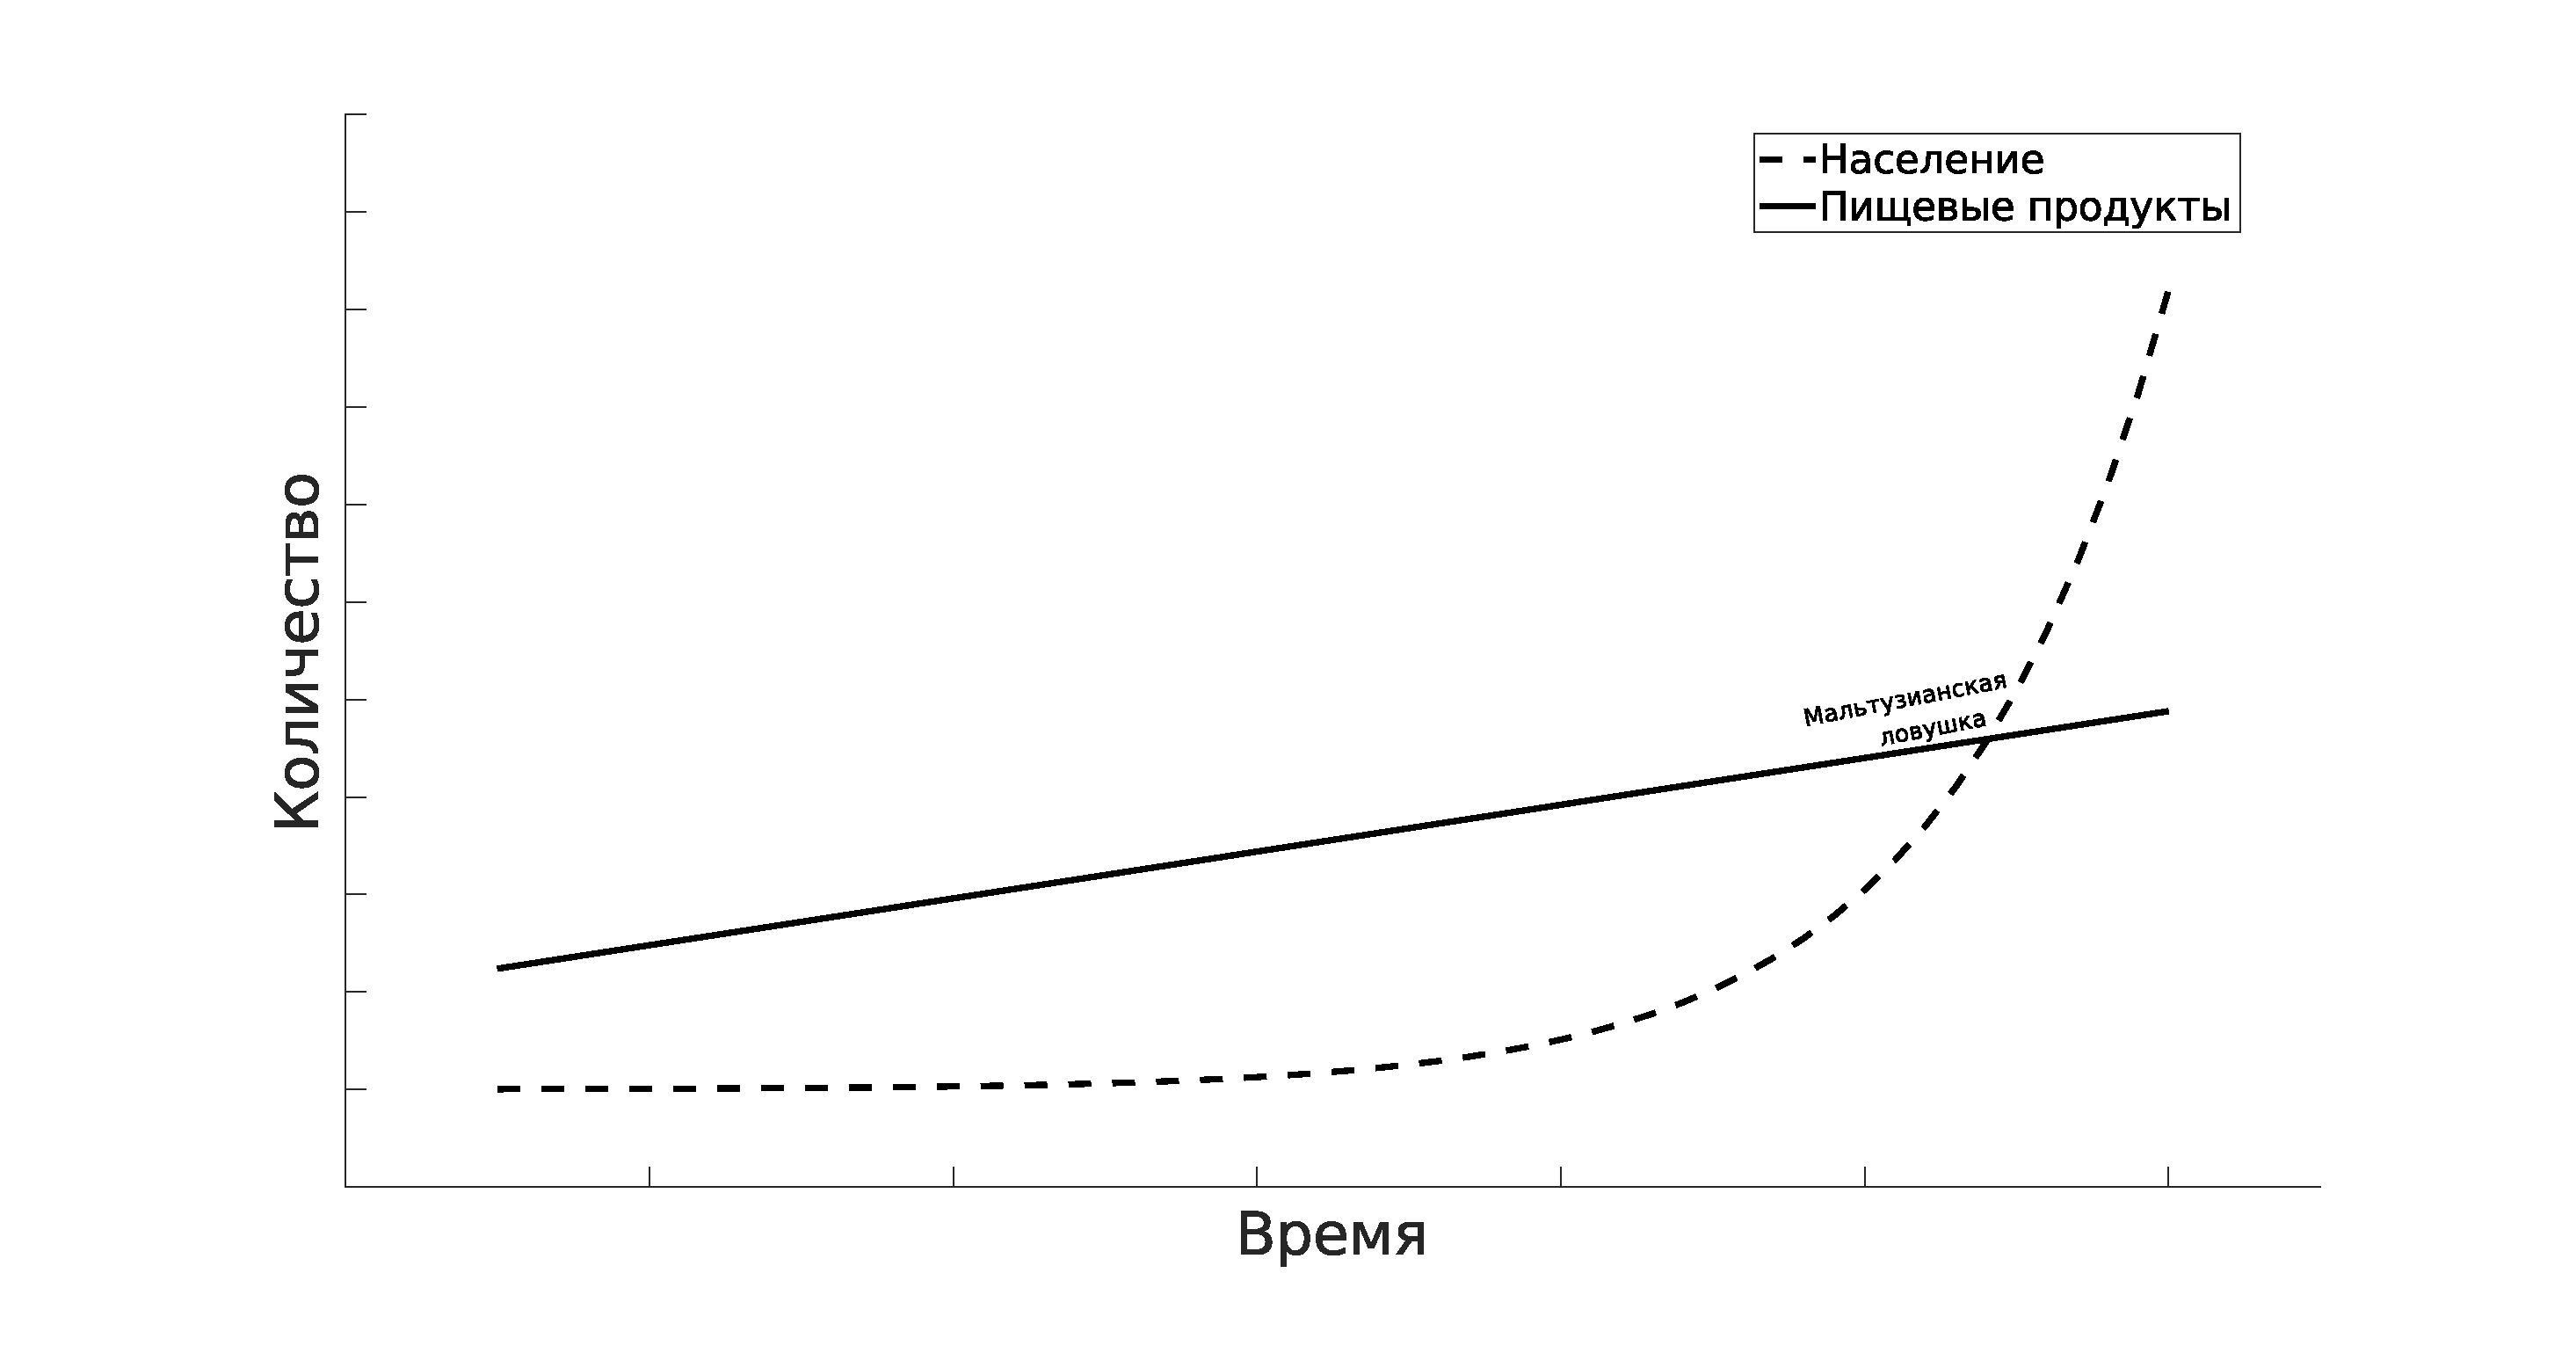
\includegraphics[width = 1.0\textwidth]{malthus.eps}
}
\caption{Мальтузианская ловушка}
\label{fig2}
\end{figure}